\section{Исследовательский раздел}
\subsection{Условия исследований}
Исследование проводилось на персональном вычислительной машине со следующими характеристиками:

\begin{itemize}
\item процессор Apple M1 Pro,
\item операционная система Ventura 13.5.2,
\item 32 Гб оперативной памяти.
\end{itemize}

Временные затраты определялись с использованием библиотеки time. Значение ROC-AUC определялось с использованием библиотеки LibRecommender.

В данном исследовании значение параметра, отвевающего за количество используемых похожих объектов, менялось от $1$ до $30$. Также для каждого алгоритма и значения параметра использовались косинусная мера, критерий Пирсона и мера Жаккара.

\subsection{Зависимости времени выполнения коллаборативной фильтрации от параметра количества используемых похожих объектов для каждой из мер близости}

На рисунке \ref{img:time1} представлен график зависимости времени выполнения коллаборативной фильтрации по пользователю от параметра количества используемых похожих объектов для каждой из мер близости.

\begin{figure}[H]
	\centering
	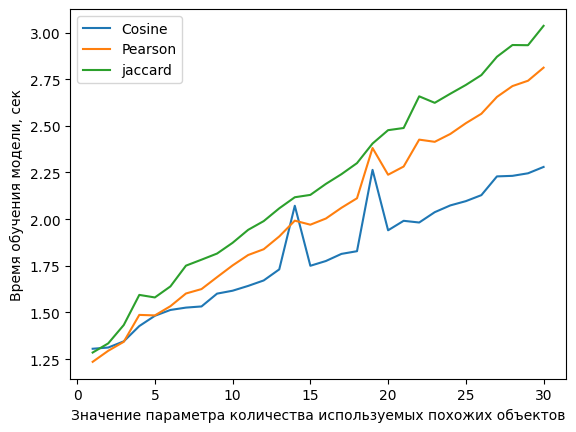
\includegraphics[width=\textwidth]{inc/timesUser.png}
	\caption{ График зависимости времени выполнения коллаборативной фильтрации по пользователю от параметра количества используемых похожих объектов для каждой из мер близости.}
	\label{img:time1}
\end{figure}

На рисунке \ref{img:time2} представлен график зависимости времени выполнения коллаборативной фильтрации по объекту от параметра количества используемых похожих объектов для каждой из мер близости.

\begin{figure}[H]
	\centering
	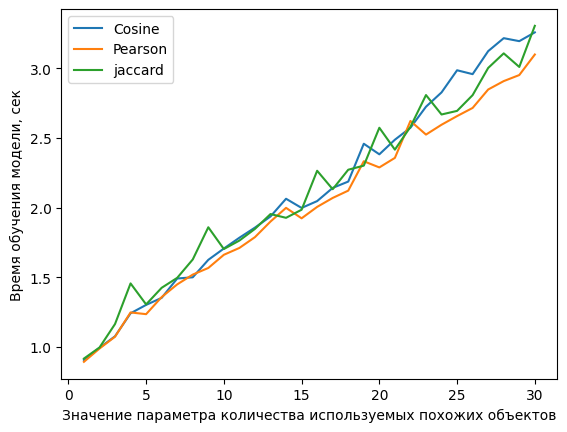
\includegraphics[width=\textwidth]{inc/timesItem.png}
	\caption{ График зависимости времени выполнения коллаборативной фильтрации по объекту от параметра количества используемых похожих объектов для каждой из мер близости.}
	\label{img:time2}
\end{figure}

\subsection{Зависимости значений ROC-AUC от параметра количества используемых похожих объектов}

На рисунке \ref{img:roc1} представлен график зависимости ROC-AUC (при фильтрации по пользователю) от параметра количества используемых похожих объектов для каждой из мер близости.

\begin{figure}[H]
	\centering
	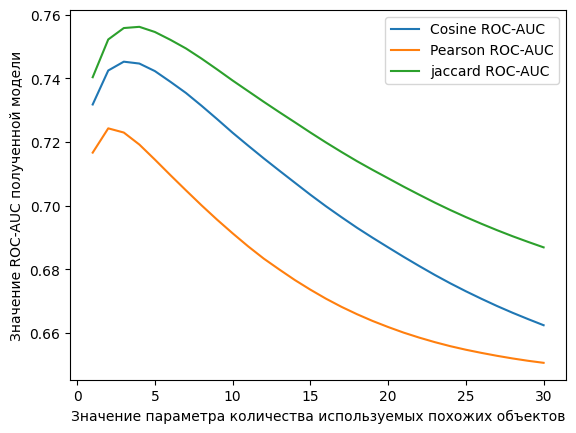
\includegraphics[width=\textwidth]{inc/rocUser.png}
	\caption{ График зависимости ROC-AUC (при фильтрации по пользователю) от параметра количества используемых похожих объектов для каждой из мер близости.}
	\label{img:roc1}
\end{figure}

На рисунке \ref{img:roc2} представлен график зависимости ROC-AUC (при фильтрации по объекту) от параметра количества используемых похожих объектов для каждой из мер близости.

\begin{figure}[H]
	\centering
	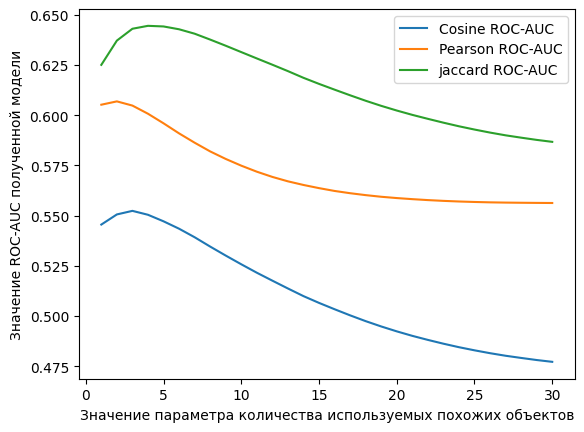
\includegraphics[width=\textwidth]{inc/rocItem.png}
	\caption{ График зависимости ROC-AUC (при фильтрации по объекту) от параметра количества используемых похожих объектов для каждой из мер близости.}
	\label{img:roc2}
\end{figure}

\subsection*{Заключение}

В результате проведенных исследований заметно, что при фильтрации по пользователю, лучше всего по времени себя показала косинусная мера на значениях параметра больше 5. В случае фильтрации по объекту, сложно выделить какую-то из мер близости.

Также стало понятно, что на рассматриваемом датасете с точки зрения ROC-AUC лучшим значением параметра количества используемых похожих объектов при фильтрации и по пользователю, и по объекту, будет находится в интервале $[3, 5]$, причем лучше всего себя показывает именно мера Жаккара.